\documentclass[twoside,twocolumn]{article}

\usepackage{blindtext} % Package to generate dummy text throughout this template 

\usepackage[sc]{mathpazo} % Use the Palatino font
\usepackage[T1]{fontenc} % Use 8-bit encoding that has 256 glyphs
\linespread{1.05} % Line spacing - Palatino needs more space between lines
\usepackage{microtype} % Slightly tweak font spacing for aesthetics
\usepackage[utf8]{inputenc}
\usepackage[english]{babel} % Language hyphenation and typographical rules

\usepackage[hmarginratio=1:1,top=32mm,columnsep=20pt]{geometry} % Document margins
\usepackage[hang, small,labelfont=bf,up,textfont=it,up]{caption} % Custom captions under/above floats in tables or figures
\usepackage{booktabs} % Horizontal rules in tables

\usepackage{lettrine} % The lettrine is the first enlarged letter at the beginning of the text

\usepackage{enumitem} % Customized lists
\setlist[itemize]{noitemsep} % Make itemize lists more compact

\usepackage{abstract} % Allows abstract customization
\renewcommand{\abstractnamefont}{\normalfont\bfseries} % Set the "Abstract" text to bold
\renewcommand{\abstracttextfont}{\normalfont\small\itshape} % Set the abstract itself to small italic text

\usepackage{titlesec} % Allows customization of titles
\renewcommand\thesection{\Roman{section}} % Roman numerals for the sections
\renewcommand\thesubsection{\roman{subsection}} % roman numerals for subsections
\titleformat{\section}[block]{\large\scshape\centering}{\thesection.}{1em}{} % Change the look of the section titles
\titleformat{\subsection}[block]{\large}{\thesubsection.}{1em}{} % Change the look of the section titles

\usepackage{fancyhdr} % Headers and footers
\pagestyle{fancy} % All pages have headers and footers
\fancyhead{} % Blank out the default header
\fancyfoot{} % Blank out the default footer
\fancyhead[C]{Running title $\bullet$ May 2016 $\bullet$ Vol. XXI, No. 1} % Custom header text
\fancyfoot[RO,LE]{\thepage} % Custom footer text

\usepackage{titling} % Customizing the title section

\usepackage{hyperref} % For hyperlinks in the PDF

\usepackage{graphicx}
\graphicspath{ {img/} }

%----------------------------------------------------------------------------------------
%	TITLE SECTION
%----------------------------------------------------------------------------------------

\setlength{\droptitle}{-4\baselineskip} % Move the title up

\pretitle{\begin{center}\Huge\bfseries} % Article title formatting
	\posttitle{\end{center}} % Article title closing formatting
\title{Content-based recommendations in~e-commerce services} % Article title
\author{%
	\textsc{John Smith}\thanks{A thank you or further information} \\[1ex] % Your name
	\normalsize Warsaw University of Technology \\ % Your institution
	\normalsize Faculty of Mathematics and Information Science \\
	\normalsize ul. Koszykowa 75 \\
	\normalsize 00-662 Warsaw, Poland \\
	\normalsize \href{mailto:john@smith.com}{john@smith.com} % Your email address
	%\and % Uncomment if 2 authors are required, duplicate these 4 lines if more
	%\textsc{Jane Smith}\thanks{Corresponding author} \\[1ex] % Second author's name
	%\normalsize University of Utah \\ % Second author's institution
	%\normalsize \href{mailto:jane@smith.com}{jane@smith.com} % Second author's email address
}
\date{\today} % Leave empty to omit a date
\renewcommand{\maketitlehookd}{%
	\begin{abstract}
			%TODO Pierwsze zdanie: zagajenie, że systemy reko są ważne
		%TODO Dalej: In this paper..
		
		Recommendation systems play an important role in modern e-commerce services. The more relevant items are presented to the user, the more likely s/he is to stay on a website and eventually make a transaction. In this paper, we adapt some state-of-the-art methods for determining similarities between text documents to content-based recommendations problem. The goal is to investigate a possibility of improving an existing recommendation system being a part of Allegro e-commerce platform using semantic text analysis methods. As a conclusion we show, that there is no significant difference between examined methods and previously used elasticsearch-based query in content-based recommendation task. 
		
	\end{abstract}
	{\bf Keywords:} recommendations, natural language processing, word embedding, semantics, allegro
	
}

%----------------------------------------------------------------------------------------

\begin{document}
	\maketitle
	%INTRODUCTION---------------------------------------------------------------------------------------------------------------------------------------
	\section{Introduction}
	
	% Po kolei wymienić metody: LSA, LDA, bengio, collobert, word2vec itp...
	%Zagajenie
	Recommendation systems are commonly used in e-commerce services. Such system give profit to both a user as well as a website owner. They allow the user to get to an information s/he could not find, or even know, that such information exists. They also attract users to a service making them more likely to buy something, increasing website company's profit thereby. The key issue of recommendations generation is how suggested items are relevant to these which the user is interested in. 
	
	%Lekkie wprowadzenie do rekomendacji
	Generally we can divide recommendation systems into two groups: collaborative and content-based filtering. The first one assumes that user is likely to be interested in items which also users similar to s/he were interested in. In this paper we are focusing on the second group in which recommended items are similar to these that the user liked so far.
	
	%O Allegro
	A detailed problem comes from the on-line auction site Allegro. Allegro --- the biggest marketplace platform in Eastern Europe --- contains a section presenting text articles concerning products available via the platform. Next to article currently displayed by a user, there is a list of links to articles similar to given one. Previous recommendations determining mechanism is based on elasticsearch query and uses both an article text and some metadata attached to the article.
	
	%Synteza: co będziemy robić z rekomendacjami w Allegro
	In this paper we strive to check if some semantic text analysis methods, including newly proposed word embeddings, are able to replace previously used Allegro method. Examined methods are topic modeling methods: latent semantic analysis~\cite{lsa}, latent Dirichlet allocation~\cite{lda} and word embeddings methods: word2vec~\cite{word2vec}, fastText~\cite{fasttext} and GloVe~\cite{glove}.
	
	%Plan artykułu
	In section 2 we make an analysis of the articles dataset and also we describe data preprocessing we performed. Section 3 is about methods used for building the model and next evaluate results. In section 4 we present the results and try to interpret them. The last section concludes the papers and proposes a direction of future work.
	%DATASET------------------------------------------------------------------------------------------------------------------------------------
	\section{Dataset}
	%TODO Skąd pochodzi zbiór danych
	
	As mentioned our dataset comes form Allegro e-commerce platform. It consists of 20000 text articles describing several categories of products available via Allegro platform. Single record consists of article contents and metadata attached by an author of the article. As significant metadata we consider ,,category'' and ,,keywords''.
	
	%krótko opisać keywords i category
	
	All articles are written in Polish. The vocabulary based on the articles set contains many industry-specific words like brands and models names, books titles and technical words. Moreover raw articles contain some tags responsible for images and hyperlinks present on the website.
	
	A standard activity before building a model is preprocessing of a raw dataset. The following enumeration describes steps of the preprocessing that we performed.
	\begin{enumerate}
		
		\item Cleansing the text from the redundant, previously mentioned tags. From the viewpoint of semantic analysis they are useless or even noxious. That is why we remove them using properly constructed regular expressions. An example of such a tag is \texttt{[2\_new.jpg] (http: // (...)'2\_new.jpg')} placing the picture in the middle of the text (the content of the URL removed due to confidentiality reasons).
		
		\item Removal of stopwords --- usually short words carrying very little information about the actual document contents, e.g. ,,in'', ,,from'', ,,because'' etc. Removing them reduces the number of words in a document and the processing time thereby.
		
		\item Converting all words of a document to lowercase letters. It helps to unify words with the same meaning, but written using both uppercase and lowercase letters.
		
		\item Breaking down the words connected with a hyphen. Experience at a later lemmatisation stage shows that the tool used to it (Morfologik~\cite{morfologik}) does not cope with these types of words and leaves them in the unchanged grammatical form. This made it necessary to build our own tool that breaks such words into sub-words compatible with the lemmatiser.
		
		\item Tokenization and lemmatisation. This is the most important element of the process. It's about separating text into individual words and converting the words with the same meaning, and different grammatical form to the same form. Complexity of the Polish language and the number of exceptions that this language has are making this problem harder than in many other languages. To carry out this operation, we used the Morfologik tool~\cite{morfologik}.
	
	\end{enumerate}
	
	The above steps lead the data to a state in which we can apply examined semantic techniques of text analysis. The dictionary built on the preprocessed corpus contains 98174 unique	words and 7409145 all words (with repetitions).	The overwhelming majority of the words of the dictionary built on the body are the words appearing rarely.
	%METHODS-------------------------------------------------------------------------------------------------------------------------------------
	\section{Methods}

	Emerging popularity of word embeddings methods started 
	
	Next we had to choose an evaluation method....

	\subsection{Model building}
	
	Below enumeration contains text analysis methods we decided to adapt for our content-based recommendations task.
	
	\begin{enumerate}
		\item Latent semantic analysis
		\item Latent Dirichlet allocation
		\item Word2Vec %We decided to train word embedding models on our dataset.
		\item GloVe
		\item FastText
	\end{enumerate}
	
	Hyperparameters of the methods...
	
	Word2Vec authors offer pretrained model but only for English language. For Polish it's more difficult...
	Lack of presumably important words like brand and model names etc.  
	
	
	%Wzmianka o usrednianiu wektorów word embeddings
	
	
	Text requiring further explanation\footnote{Example footnote}.
	
	\subsection{Evaluation}
	
	In order to compare the methods used to determine the similarity between the articles, the formalization of certain measures of this similarity seems necessary.
	
	
	In practice, however, it is rarely worth the value of a given element of the ranking
	is adequate to the query generating this ranking.
	
	Evaluation of recommendations generation methods is a nontrivial task. A degree of similarity of two articles can be perceived differently by different persons. Therefore we decided to evaluate methods' performance with .... First with each tested method we choose 6 most similar articles for 50 randomly chosen base articles. Next we split them into pairs: base article --- similar article; it gave us $5*50=250$ pairs for a method. After that 5 persons individually evaluated a similarity of pairs of articles giving scores in scale 1-10. Finally we took an average score for each pair and it allowed us to calculate an average score for each method. Besides tested methods we evaluated also previous Allegro method and randomly generated pairs of articles just for a comparison purpose.
	
	
	
	%RESULTS & DISCUSSION-----------------------------------------------------------------------------------------------------------------------------------------------------------
	\section{Results and discussion}
	In order to compare aforementioned methods we performed described expert evaluation. The evaluated methods were: LSA, LDA, word2vec, GloVe, FastText, previous Allegro elasticsearch-based method and randomly chosen pairs of articles.


	\begin{figure}
		\centering
		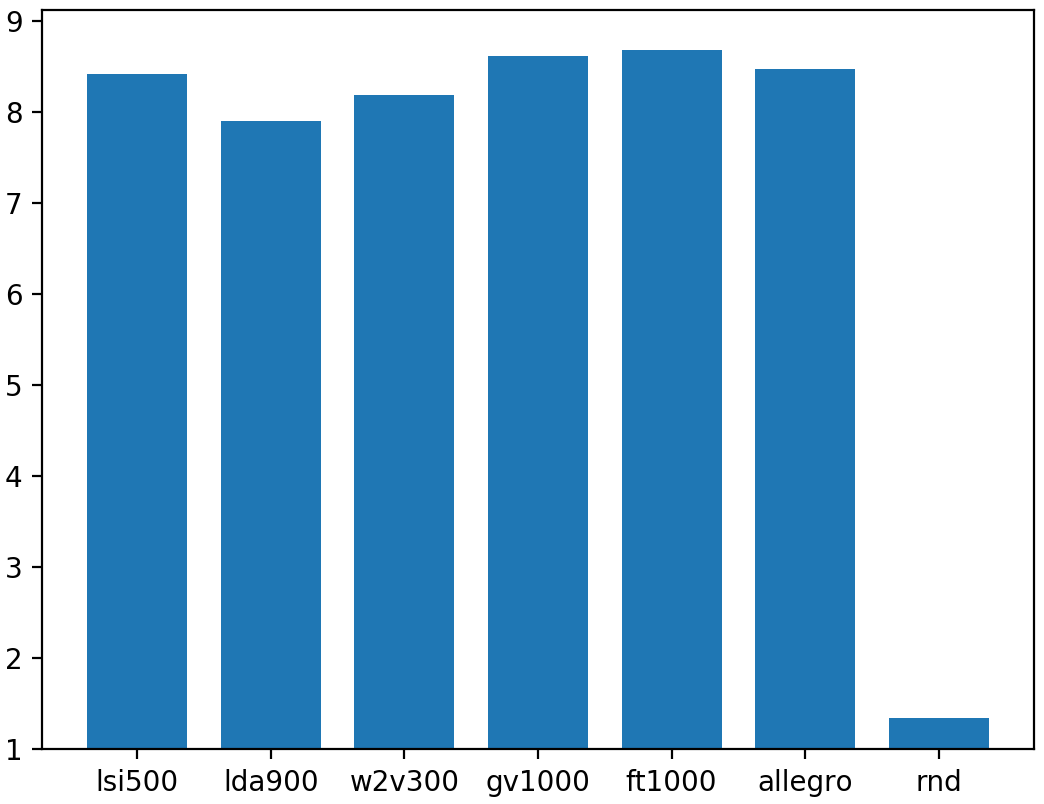
\includegraphics[width=0.45\textwidth]{results.png}
		\caption{}
		%\label{fig:warstwy}
	\end{figure}
	
	Expert evaluation suggests that none of the tested methods is significantly different from others. The difference between the best method (FastText) and the worst one (LDA) is around 9\%. Each of the tested methods also gave a significantly better result than the random method.
	
	
	To answer the question posed at the beginning of this work, i.e. whether the examined text analysis methods adapted to content-based recommendation task are able to match the previous method used in Allegro, we perform a test that's goal is to check whether there are grounds to believe that the results of any of the methods is statistically significantly different from the rest of the examined methods.
		
		
	The statistical test that we carry out is the Kruskal-Wallis test. In the test the null hypothesis $H_0$ assumes an equality of distributions in populations from which samples originated.	As input data the Kruskal-Wallis test takes samples corresponding to expert evaluation of each method consisting of an average score made by users for the most relevant recommendation for each of the examined base articles.


	In the test, the level of significance is $\alpha = 0.05$. Finally, as the result of the Kruskal-Wallis test we received $p = 0.0571>\alpha$, on the basis of which we state that there are no reasons to reject the null hypothesis --- the quality difference between of recommendations generated by the tested methods is not statistically significant. It means that neither of the tested semantic methods sticks out from others, nor the previous Allegro method is significantly better/worse than other tested methods.
	
	%CONCLUSION--------------------------------------------------------------------------------------------------------------------------------------------------------------------
	\section{Conclusion}
	
	After analyzing the test results we can answer: yes, each of the examined methods of natural language semantic analysis in their best configuration can be adapted to generate article content-based recommendations. This means we can replace previously used method with e.g. FastText and any user should not feel any difference in recommendations quality.
	
	Using methods of semantic text analysis allows to capture the hidden similarities between documents, where the documents combine not the same words or synonyms, but some abstract concepts related to each other. An important advantage of semantic methods compared to the previous one is the fact that they are based only on article contents. This frees the authors of the articles from providing additional metadata, which the previous method uses in large extent.
	
	
	\begin{thebibliography}{99}
		\bibitem{lda}
		D. M. Blei, A. Y. Ng, M. I. Jordan,
		\emph{Latent Dirichlet Allocation},
		Journal of Machine Learning Research, tom 3 num. 4–5,
		2003
		
		\bibitem{lsa}
		S. Deerwester, S. T. Dumais, G. W. Furnas, T. K. Landauer, R. Harshman,
		\emph{Indexing by latent semantic analysis},
		Journal of the American Society for Information Science, tom 41, num. 6,
		1990
		
		\bibitem{fasttext}
		A. Joulin, E. Grave, P. Bojanowski T. Mikolov,
		\emph{Bag of Tricks for Efficient Text Classification},
		Facebook AI Research,
		2016
		
		\bibitem{wmd}
		M. J. Kusner, Y. Sun, N. I. Kolkin, K. Q. Weinberger,
		\emph{From Word Embeddings To Document Distances},
		International Conference on Machine Learning (ICML),
		2015
		
		\bibitem{word2vec}
		T. Mikolov, K. Chen, G. Corrado, J. Dean,
		\emph{Efficient Estimation of Word Representations in Vector Space},
		International Conference on Machine Learning (ICML),
		2013
		
		\bibitem{morfologik}
		Morfologik
		\url{http://morfologik.blogspot.com/}
		(dostęp 07.05.2017)
		
		\bibitem{glove}
		J. Pennington, R. Socher, C. D. Manning,
		\emph{GloVe: Global Vectors for Word Representation},
		Computer Science Department, Stanford University, Stanford, CA 94305,
		2014

		
	\end{thebibliography}
	
	%----------------------------------------------------------------------------------------
	
\end{document}
.